% Options for packages loaded elsewhere
\PassOptionsToPackage{unicode}{hyperref}
\PassOptionsToPackage{hyphens}{url}
%
\documentclass[
]{article}
\usepackage{amsmath,amssymb}
\usepackage{lmodern}
\usepackage{ifxetex,ifluatex}
\ifnum 0\ifxetex 1\fi\ifluatex 1\fi=0 % if pdftex
  \usepackage[T1]{fontenc}
  \usepackage[utf8]{inputenc}
  \usepackage{textcomp} % provide euro and other symbols
\else % if luatex or xetex
  \usepackage{unicode-math}
  \defaultfontfeatures{Scale=MatchLowercase}
  \defaultfontfeatures[\rmfamily]{Ligatures=TeX,Scale=1}
\fi
% Use upquote if available, for straight quotes in verbatim environments
\IfFileExists{upquote.sty}{\usepackage{upquote}}{}
\IfFileExists{microtype.sty}{% use microtype if available
  \usepackage[]{microtype}
  \UseMicrotypeSet[protrusion]{basicmath} % disable protrusion for tt fonts
}{}
\makeatletter
\@ifundefined{KOMAClassName}{% if non-KOMA class
  \IfFileExists{parskip.sty}{%
    \usepackage{parskip}
  }{% else
    \setlength{\parindent}{0pt}
    \setlength{\parskip}{6pt plus 2pt minus 1pt}}
}{% if KOMA class
  \KOMAoptions{parskip=half}}
\makeatother
\usepackage{xcolor}
\IfFileExists{xurl.sty}{\usepackage{xurl}}{} % add URL line breaks if available
\IfFileExists{bookmark.sty}{\usepackage{bookmark}}{\usepackage{hyperref}}
\hypersetup{
  pdftitle={Bee-Wing Geometric Morphometric},
  pdfauthor={Hannes Oberreiter, 01619771},
  hidelinks,
  pdfcreator={LaTeX via pandoc}}
\urlstyle{same} % disable monospaced font for URLs
\usepackage[margin=1in]{geometry}
\usepackage{longtable,booktabs,array}
\usepackage{calc} % for calculating minipage widths
% Correct order of tables after \paragraph or \subparagraph
\usepackage{etoolbox}
\makeatletter
\patchcmd\longtable{\par}{\if@noskipsec\mbox{}\fi\par}{}{}
\makeatother
% Allow footnotes in longtable head/foot
\IfFileExists{footnotehyper.sty}{\usepackage{footnotehyper}}{\usepackage{footnote}}
\makesavenoteenv{longtable}
\usepackage{graphicx}
\makeatletter
\def\maxwidth{\ifdim\Gin@nat@width>\linewidth\linewidth\else\Gin@nat@width\fi}
\def\maxheight{\ifdim\Gin@nat@height>\textheight\textheight\else\Gin@nat@height\fi}
\makeatother
% Scale images if necessary, so that they will not overflow the page
% margins by default, and it is still possible to overwrite the defaults
% using explicit options in \includegraphics[width, height, ...]{}
\setkeys{Gin}{width=\maxwidth,height=\maxheight,keepaspectratio}
% Set default figure placement to htbp
\makeatletter
\def\fps@figure{htbp}
\makeatother
\setlength{\emergencystretch}{3em} % prevent overfull lines
\providecommand{\tightlist}{%
  \setlength{\itemsep}{0pt}\setlength{\parskip}{0pt}}
\setcounter{secnumdepth}{5}
\usepackage{hyperref}
\usepackage{float}
\usepackage{caption}
\captionsetup[figure]{font=scriptsize}
\usepackage{siunitx}
\usepackage{threeparttable}
\usepackage{booktabs}
\usepackage{longtable}
\usepackage{array}
\usepackage{multirow}
\usepackage{wrapfig}
\usepackage{float}
\usepackage{colortbl}
\usepackage{pdflscape}
\usepackage{tabu}
\usepackage{threeparttable}
\usepackage{threeparttablex}
\usepackage[normalem]{ulem}
\usepackage{makecell}
\usepackage{xcolor}
\ifluatex
  \usepackage{selnolig}  % disable illegal ligatures
\fi
\newlength{\cslhangindent}
\setlength{\cslhangindent}{1.5em}
\newlength{\csllabelwidth}
\setlength{\csllabelwidth}{3em}
\newenvironment{CSLReferences}[2] % #1 hanging-ident, #2 entry spacing
 {% don't indent paragraphs
  \setlength{\parindent}{0pt}
  % turn on hanging indent if param 1 is 1
  \ifodd #1 \everypar{\setlength{\hangindent}{\cslhangindent}}\ignorespaces\fi
  % set entry spacing
  \ifnum #2 > 0
  \setlength{\parskip}{#2\baselineskip}
  \fi
 }%
 {}
\usepackage{calc}
\newcommand{\CSLBlock}[1]{#1\hfill\break}
\newcommand{\CSLLeftMargin}[1]{\parbox[t]{\csllabelwidth}{#1}}
\newcommand{\CSLRightInline}[1]{\parbox[t]{\linewidth - \csllabelwidth}{#1}\break}
\newcommand{\CSLIndent}[1]{\hspace{\cslhangindent}#1}

\title{Bee-Wing Geometric Morphometric}
\usepackage{etoolbox}
\makeatletter
\providecommand{\subtitle}[1]{% add subtitle to \maketitle
  \apptocmd{\@title}{\par {\large #1 \par}}{}{}
}
\makeatother
\subtitle{University of Graz, Institut for Biology}
\author{Hannes Oberreiter, 01619771}
\date{}

\begin{document}
\maketitle

\hypertarget{introduction}{%
\section{Introduction}\label{introduction}}

European Honeybees, \emph{Apis mellifera}, are highly efficient pollinators of crops and wild flowers and hence provide exceptionally important economical and ecosystem services for us humans (\protect\hyperlink{ref-kearns1998}{Kearns, Inouye, and Waser 1998}; \protect\hyperlink{ref-gallai2009}{Gallai et al. 2009}). There are many subspecies and knowledge about origin and taxonomic differences and local distribution are crucial too understand them (\protect\hyperlink{ref-ruttner1988}{Ruttner 1988}; \protect\hyperlink{ref-phylogen2020}{Ilyasov and Kwon 2020}). Sadly, even though we learn each day more about importance of insect in our ecosystem a alarming decline of wild pollinators can be seen over the last years (\protect\hyperlink{ref-hallmann2017}{Hallmann et al. 2017}; \protect\hyperlink{ref-suxe1nchez-bayo2019}{Sánchez-Bayo and Wyckhuys 2019}). The reasons for the decline seem manifold: parasites; pathogens; environmental pollution; rapid climate change, loss of insect friendly habitats etc. (\protect\hyperlink{ref-biesmeijer2006}{Biesmeijer 2006}; \protect\hyperlink{ref-potts2010}{Potts et al. 2010}; \protect\hyperlink{ref-goulson2013}{Goulson 2013}; \protect\hyperlink{ref-woodcock2017}{Woodcock et al. 2017}).

In this small paper, which is part of the homework assessment for the course ``Mod. Multivariate Biostatistik und geometrische Morphometrie'' at the University of Graz I try to apply basic geometric morphometrics practices to differentiate possible subpopulations or lineages of \emph{A. m.,} similar real studies were done before and showed great success (\protect\hyperlink{ref-kandemir2009}{Kandemir et al. 2009}; \protect\hyperlink{ref-tofilski2008}{Tofilski 2008}; \protect\hyperlink{ref-francoy2006}{Francoy et al. 2006}). These studies and in my homework the fore- and backwing of \emph{A. m.} are used, as they are a easy to dissect and photograph and posses a high degree of variability in wing venation (\protect\hyperlink{ref-grimaldi2005}{Grimaldi et al. 2005}).

The main goal was to get a better understand for geometric morphometrics and how to use it in various biology questions. With the help of geometric morphometrics we can not only measure morphological similarity or differences but also put the results in the form of actual shapes in context (\protect\hyperlink{ref-mitteroecker2009}{Mitteroecker and Gunz 2009}). Other advantages of geometric morphometrics are that the data can easily collected in from digital images and size is mathematical removed with the procusters method to focus purely on shape or with size-and-shape we analyze the form (\protect\hyperlink{ref-mitteroecker2009}{Mitteroecker and Gunz 2009}; \protect\hyperlink{ref-mitteroecker2013}{Mitteroecker et al. 2013}). This would not be possible with traditional morphometrics, which is only a indirect capture of the shape.

\hypertarget{material-and-methods}{%
\section{Material and Methods}\label{material-and-methods}}

In total 52 scanned forewing and backwing images were available to me, of these, ten were given by Dr.~Robert Brodschneider, which were collected in 2011 in Graz by a student of his. Dr.~Juergen Herler, University of Vienna, did contribute the other images, which were collected in the year 2009 from colonies in Graz, Frohnleiten and Vienna. No further information on the images were given. Not all images could be used as I only used wings were all landmarks were visible also the backwing scans for Graz 2011 had a really poor quality and were dropped and not analyzed.

Landmarks (LM) were set on homologous points either at the end of wing veins or were two or more veins met, this was done with the tps software package (\protect\hyperlink{ref-rohlf2015}{Rohlf 2015}), the set landmarks can be seen in figure \ref{fig:landmarkImage}. Analysis was performed in R with the RStudio IDE and tidyverse (\protect\hyperlink{ref-r2020}{R Core Team 2020}; \protect\hyperlink{ref-RStudio2021}{RStudio Team 2021}; \protect\hyperlink{ref-tidyverse2019}{Wickham et al. 2019}). Generalized procuster analysis (GPA), which centers the shape on the origin, scales all shape to the unit size of one and tries to minimize least square distance by roation (\protect\hyperlink{ref-mitteroecker2009}{Mitteroecker and Gunz 2009}), was performed with the \protect\hyperlink{ref-geomorph2021a}{Adams et al.} (\protect\hyperlink{ref-geomorph2021a}{2021}) package. Also the setting of sliding landmarks and thin-plate spline (TPS) deformation grids were done with \protect\hyperlink{ref-geomorph2021a}{Adams et al.} (\protect\hyperlink{ref-geomorph2021a}{2021}). The resulting aligned procuster coordinates, which represents the shape for each specimen, were exploratory analyzed with principal component analysis (PCA) and also used to extract the point-distance (\protect\hyperlink{ref-raster2020}{Hijmans 2020}) to calculate the traditional morphometrics cubital index (CI) based on \protect\hyperlink{ref-goetze1959}{Goetze} (\protect\hyperlink{ref-goetze1959}{1959}). For the multiple group linear discriminant analysis or canonical variate analysis (CVA) the first ten principal components (PC) were used, accuracy of classification was tested with leave-one-out cross-validation (\protect\hyperlink{ref-MASS2002}{Venables and Ripley 2002}).



\begin{figure}[H]

{\centering 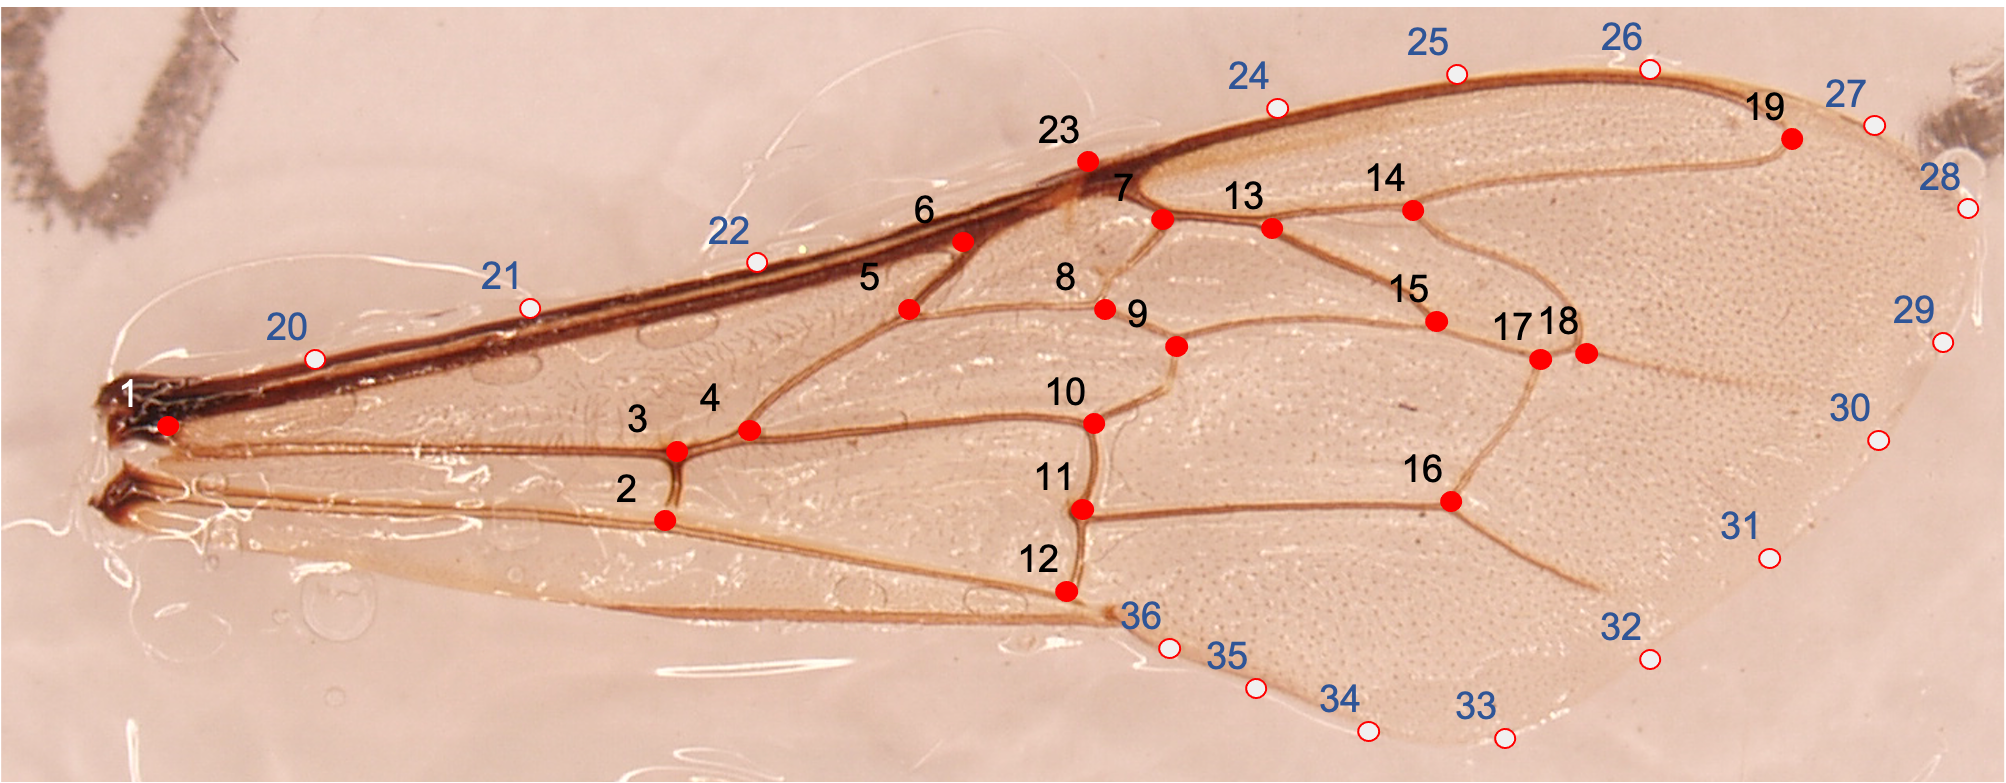
\includegraphics[width=0.4\linewidth,]{images/forewing} 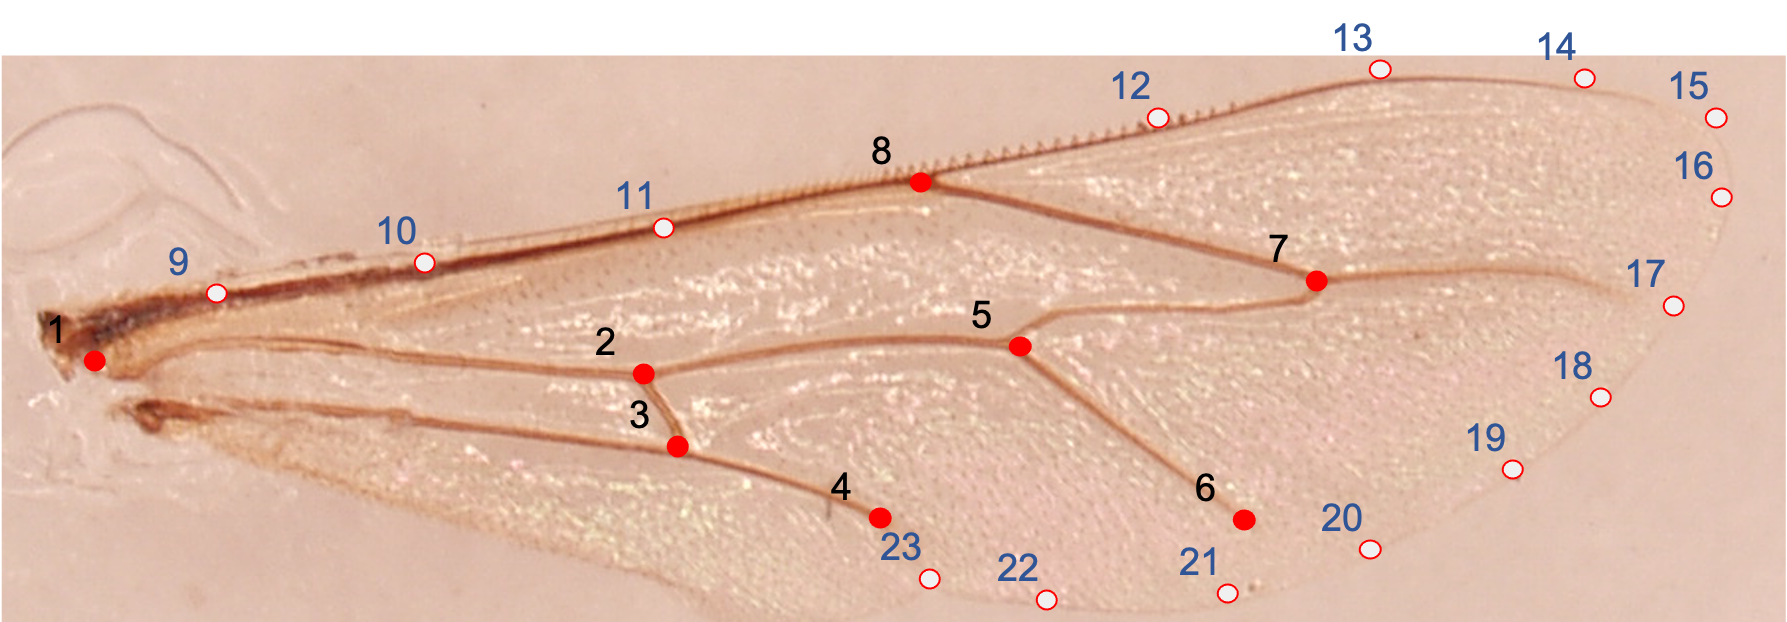
\includegraphics[width=0.4\linewidth,]{images/backwing} 

}

\caption{Example of forewing (left) and backwing (right) image, with landmark positions. White colored points with blue numbers represent the appr. location of the sliding landmarks, which define the outline of the wing.}\label{fig:landmarkImage}
\end{figure}

\hypertarget{results}{%
\section{Results}\label{results}}



\begin{figure}[H]

{\centering 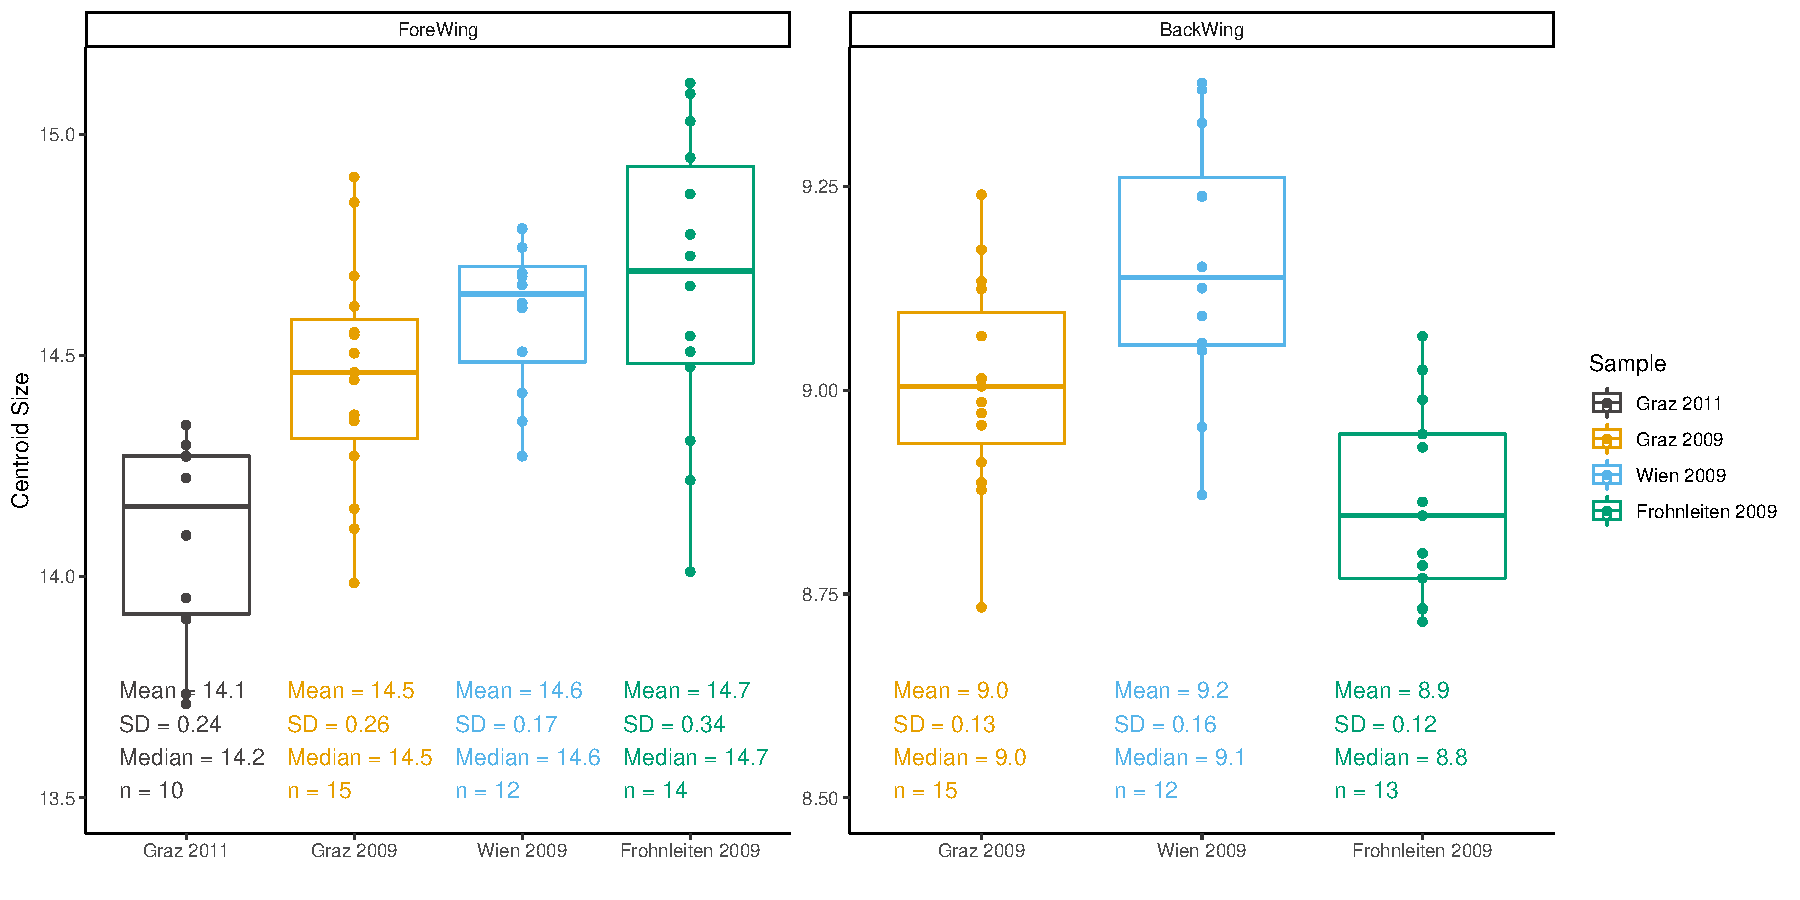
\includegraphics[width=0.7\linewidth,]{images/csPlot} 

}

\caption{Boxplot distribution of the centroid size. Comparison between samples forewing and backwing respectively. Backwing is missing for ``Graz 2011'' due to poor image quality.}\label{fig:csPlot}
\end{figure}

The measure of overall size with centroid size, which is the sum of distances from landmarks to centroid, shows clear inter-sample difference between all groups for the forewing, see figure \ref{fig:csPlot} - left. The sample ``Graz 2011'' shows on average lowest centroid size. Highest on average, but also with widest standard deviation, is the sample ``Frohnleiten 2009.'' The backwing shows also difference between the groups, sample ``Graz 2011'' is missing due to poor image quality, see figure \ref{fig:csPlot} - right. For the backwing the sample ``Frohnleiten 2009'' has the smallest centroid size on average, compared to the other two groups.



\begin{figure}[H]

{\centering 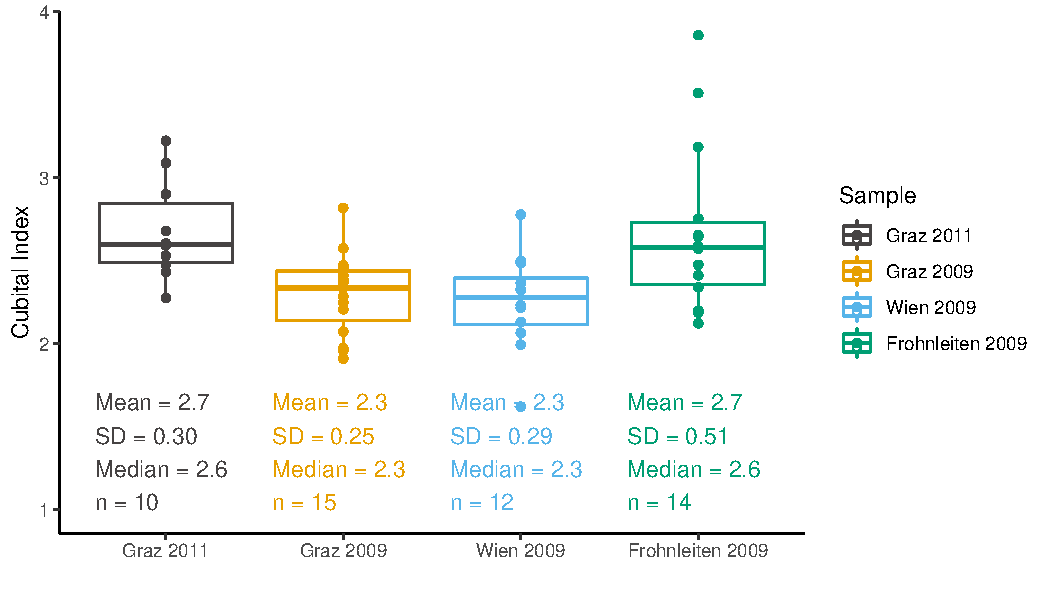
\includegraphics[width=0.6\linewidth,]{images/ciPlot} 

}

\caption{Boxplot distribution of the traditional forewing cubital index (CI) (\protect\hyperlink{ref-goetze1959}{Goetze 1959}). The CI was calculated by the point distance between LM 15-17 divided by the point distance between LM 17-18, see figure \ref{fig:landmarkImage}.}\label{fig:ciPlot}
\end{figure}

The comparison of distribution and central tendency of the traditional cubital index (CI) (\protect\hyperlink{ref-goetze1959}{Goetze 1959}) is similar between the samples, see figure \ref{fig:ciPlot}. No clear inter-sample differentiation of all groups, with CI alone, would be possible.



\begin{figure}[H]

{\centering 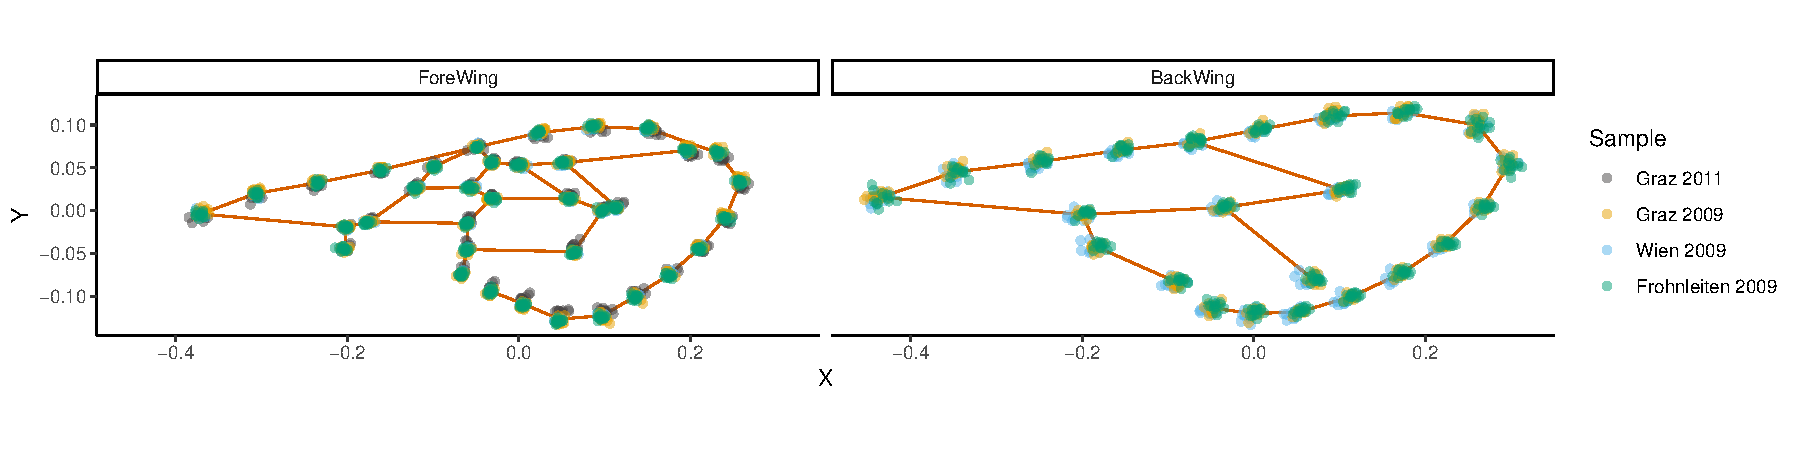
\includegraphics[width=1\linewidth,]{images/pcPlot} 

}

\caption{Aligned procuster coordinates for all specimens, after GPA. Links (red lines), to better visualize the shape, are connected on the mean coordinates.}\label{fig:pcPlot}
\end{figure}

The landmark (LM) position after GPA for all specimens can be seen in fig.~\ref{fig:pcPlot}. Backwing shows more variation of the aligned procuster coordinates, compared to the forewing.



\begin{figure}[H]

{\centering 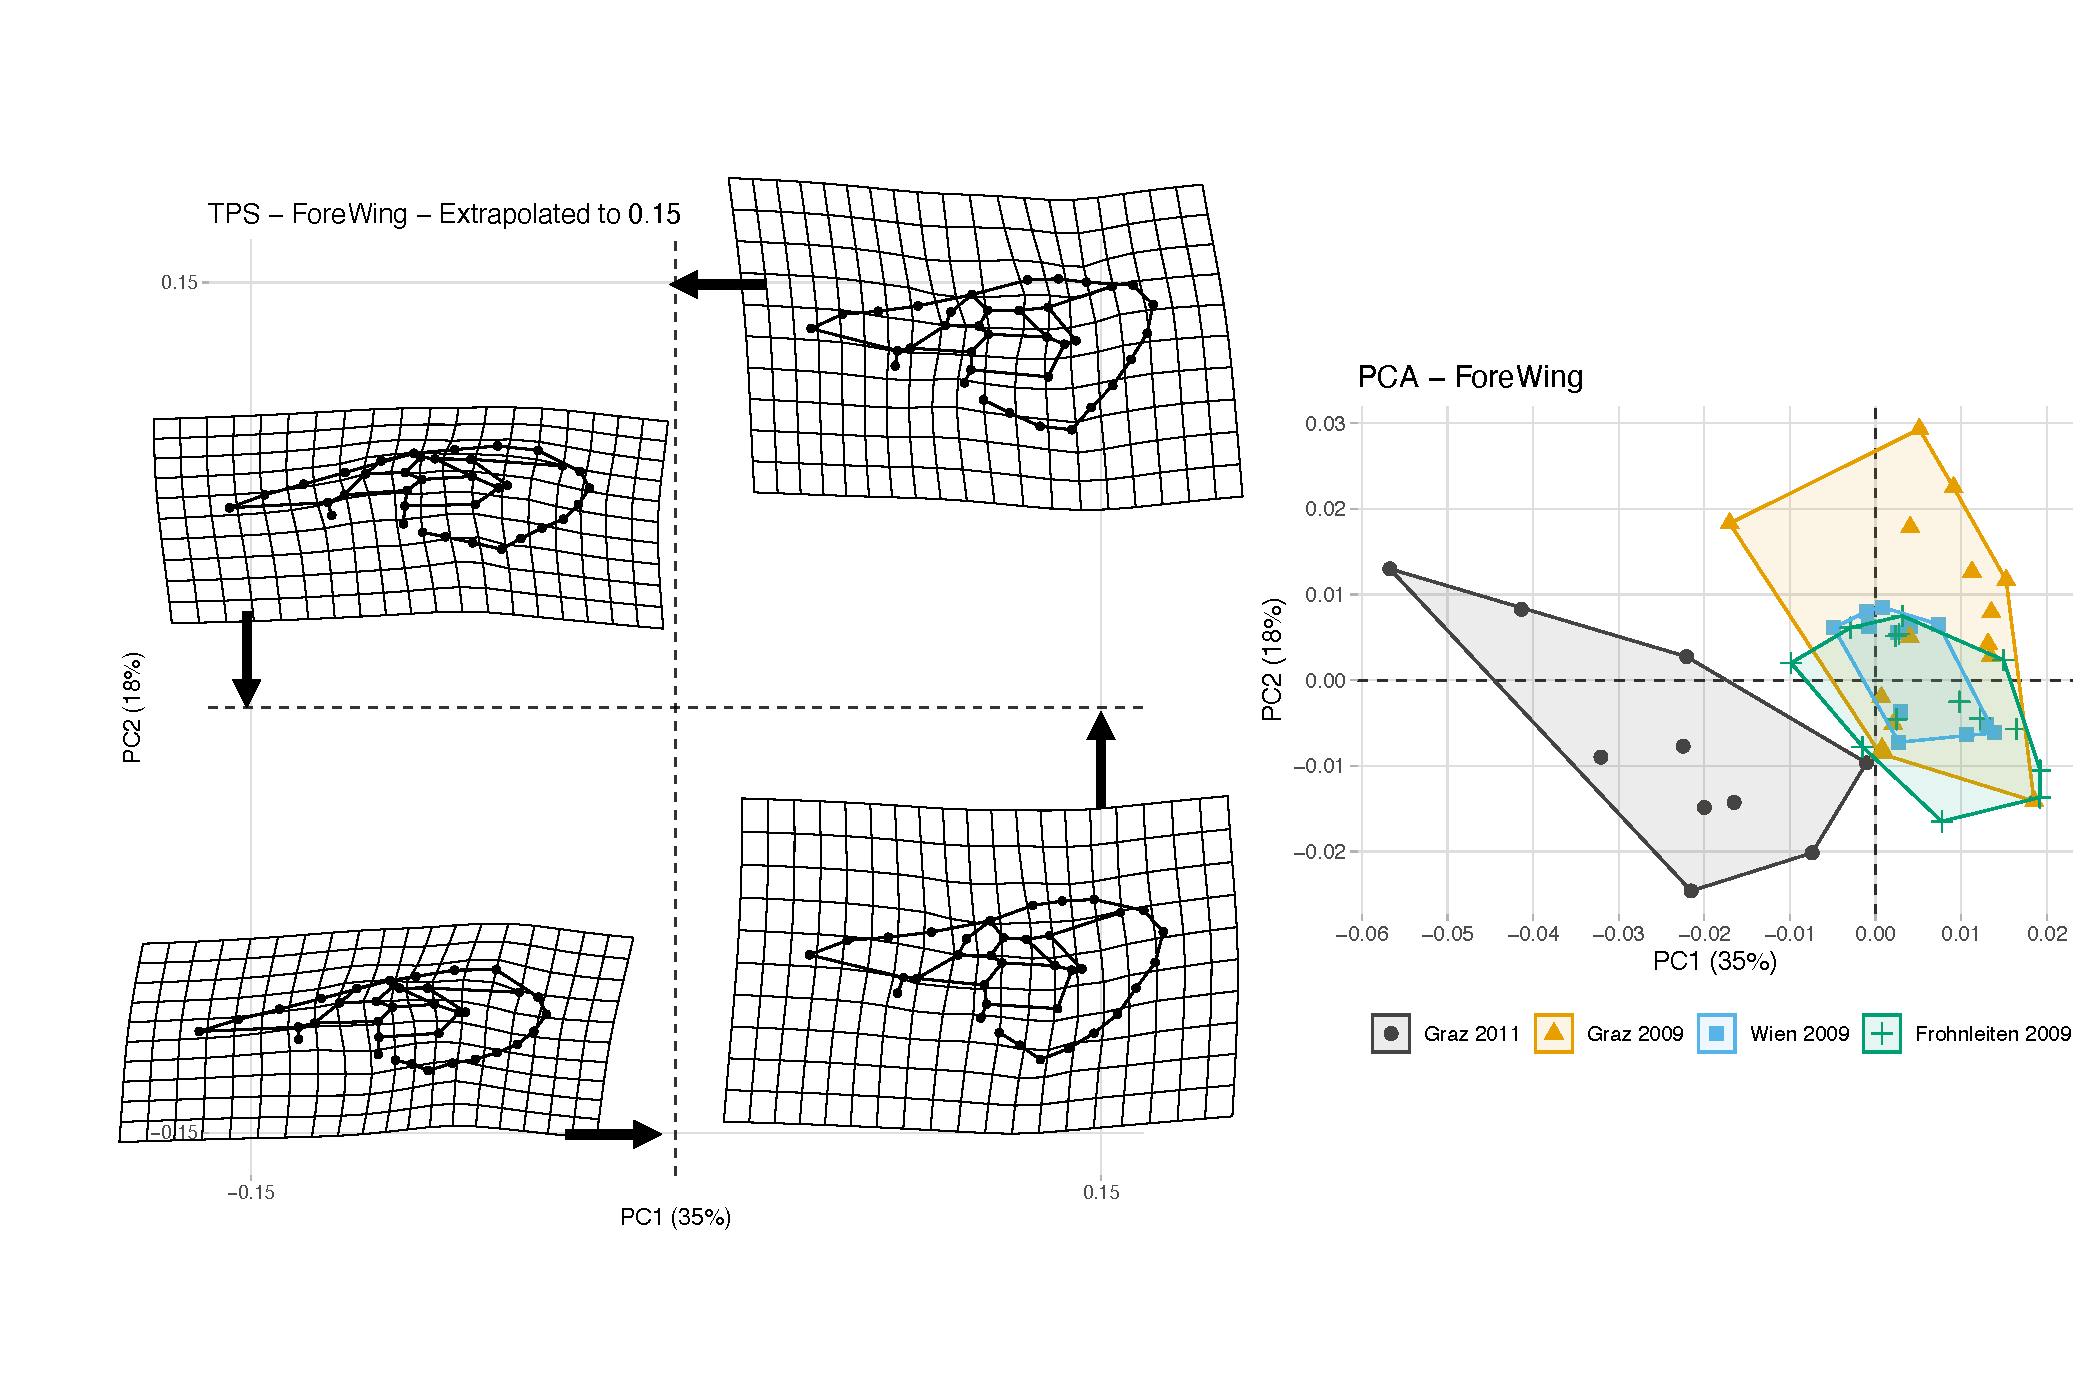
\includegraphics[width=0.8\linewidth,]{images/fwPCA} 

}

\caption{Forewing PC1 and PC2 on aligned procuster coordinates and TPS of the extrapolated PC axis difference to the mean reference shape of all specimen.}\label{fig:fwPCA}
\end{figure}

The PCA for the forewing separates on the first PC the ``Graz 2011'' sample from the rest, see \ref{fig:fwPCA}. The first PC does already explain over a third of the total variance of all principal components. The first and second combined already over 50\% of the total variance, see fig.~The shape change to the mean reference for the first PC indicates that the sample from ``Graz 2011'' has a more slimmer shape. Also the second PC has the same overall shape difference, but vein distances between other landmarks are different.



\begin{figure}[H]

{\centering 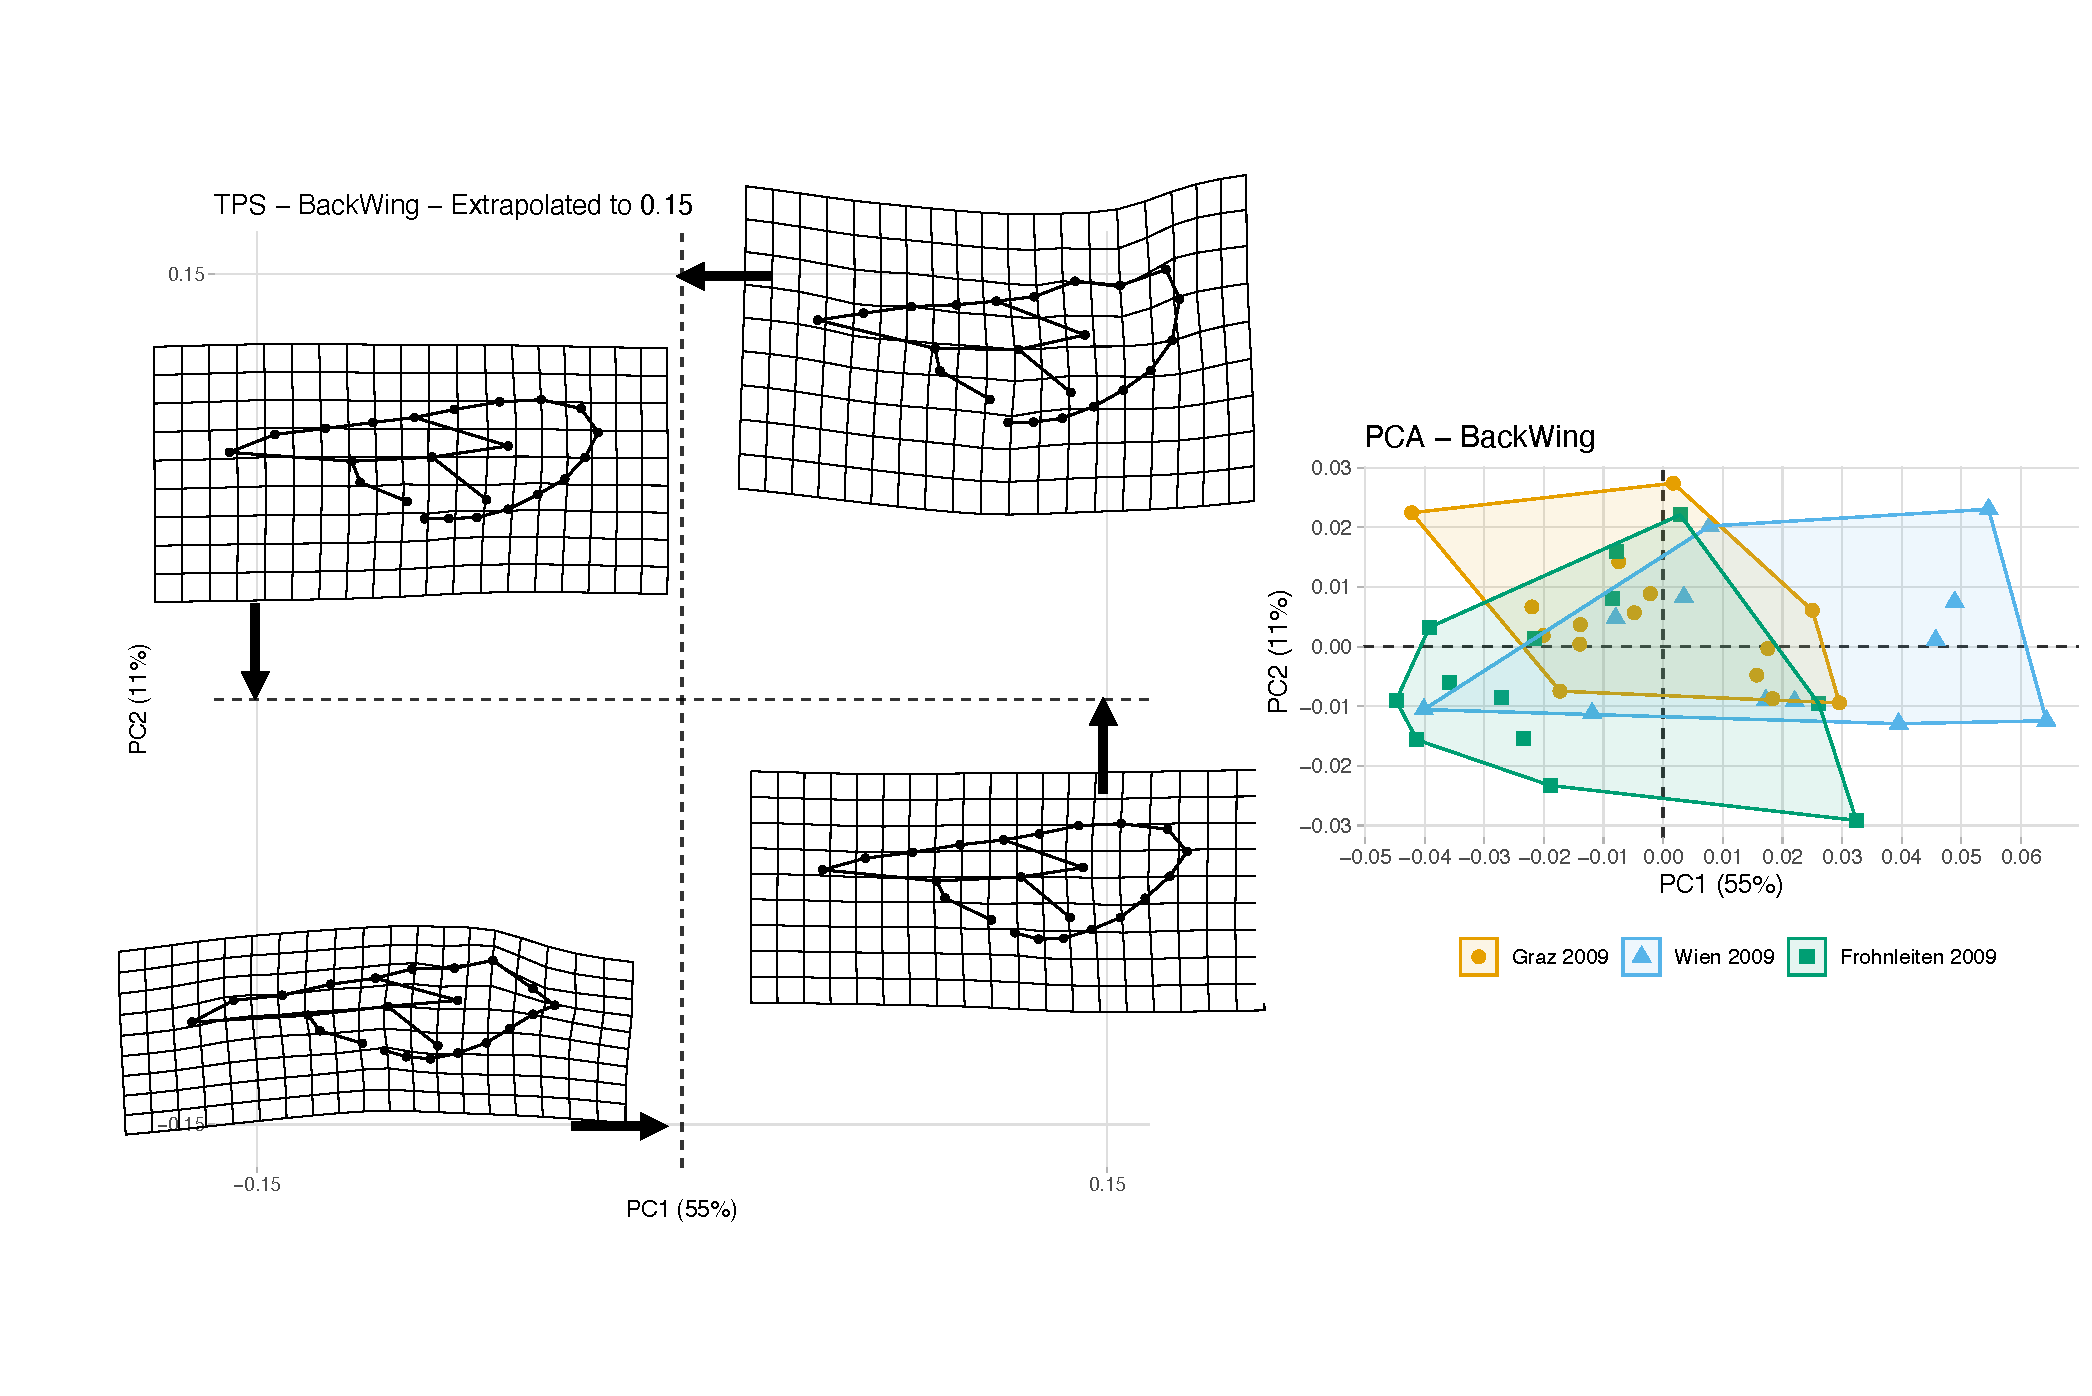
\includegraphics[width=0.8\linewidth,]{images/bwPCA} 

}

\caption{Backwing PC1 and PC2 on aligned procuster coordinates and TPS of the extrapolated PC axis difference to the mean reference shape of all specimen.}\label{fig:bwPCA}
\end{figure}

As for the backwing only the samples from the year 2009 are included and also only a subset as not all backwings were complete. All groups are overlapping in the first two dimensions, which cumulative can explain 66\% of the total variance, see fig.~\ref{fig:bwPCA}. The shape of the first PC differentiate mainly in total vertical volume of the radial cell. Both first and second PC are predominately defined by the difference of sliding landmarks.



\begin{figure}[H]

{\centering 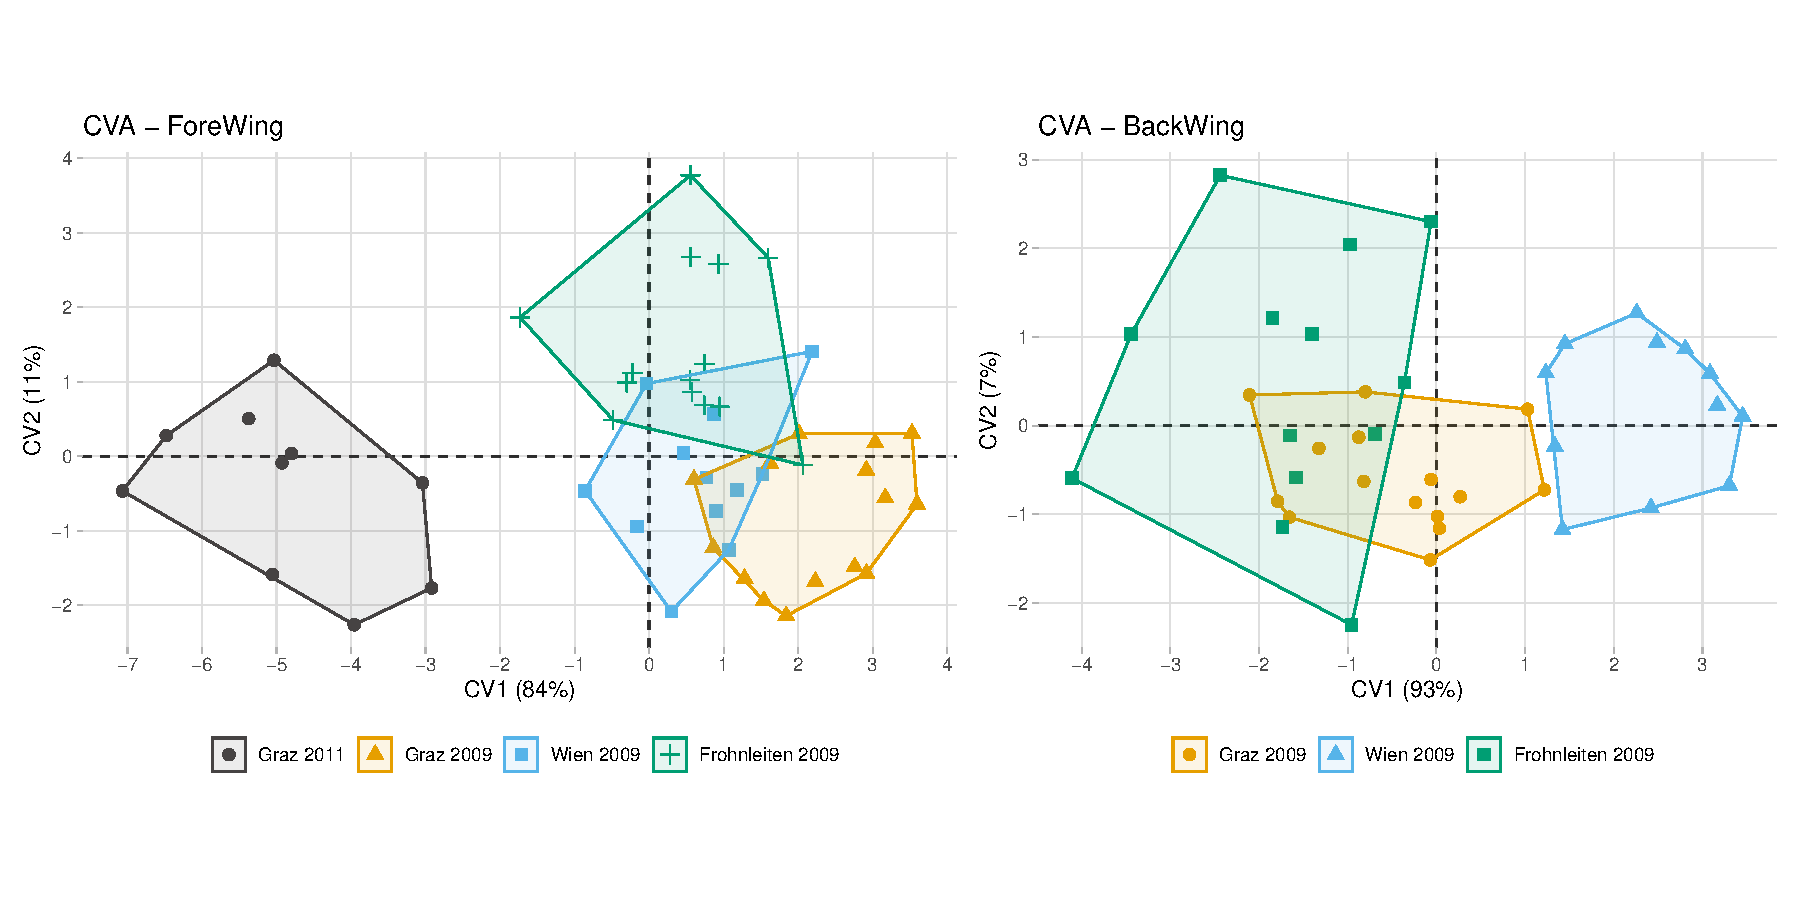
\includegraphics[width=1\linewidth,]{images/cvaPlot} 

}

\caption{Exploratory CVA based on the 1-10 PC for forewing and backwing respectively. The percent of captured between-group variance is given on the axes.}\label{fig:CVA}
\end{figure}



\begin{figure}[H]

{\centering 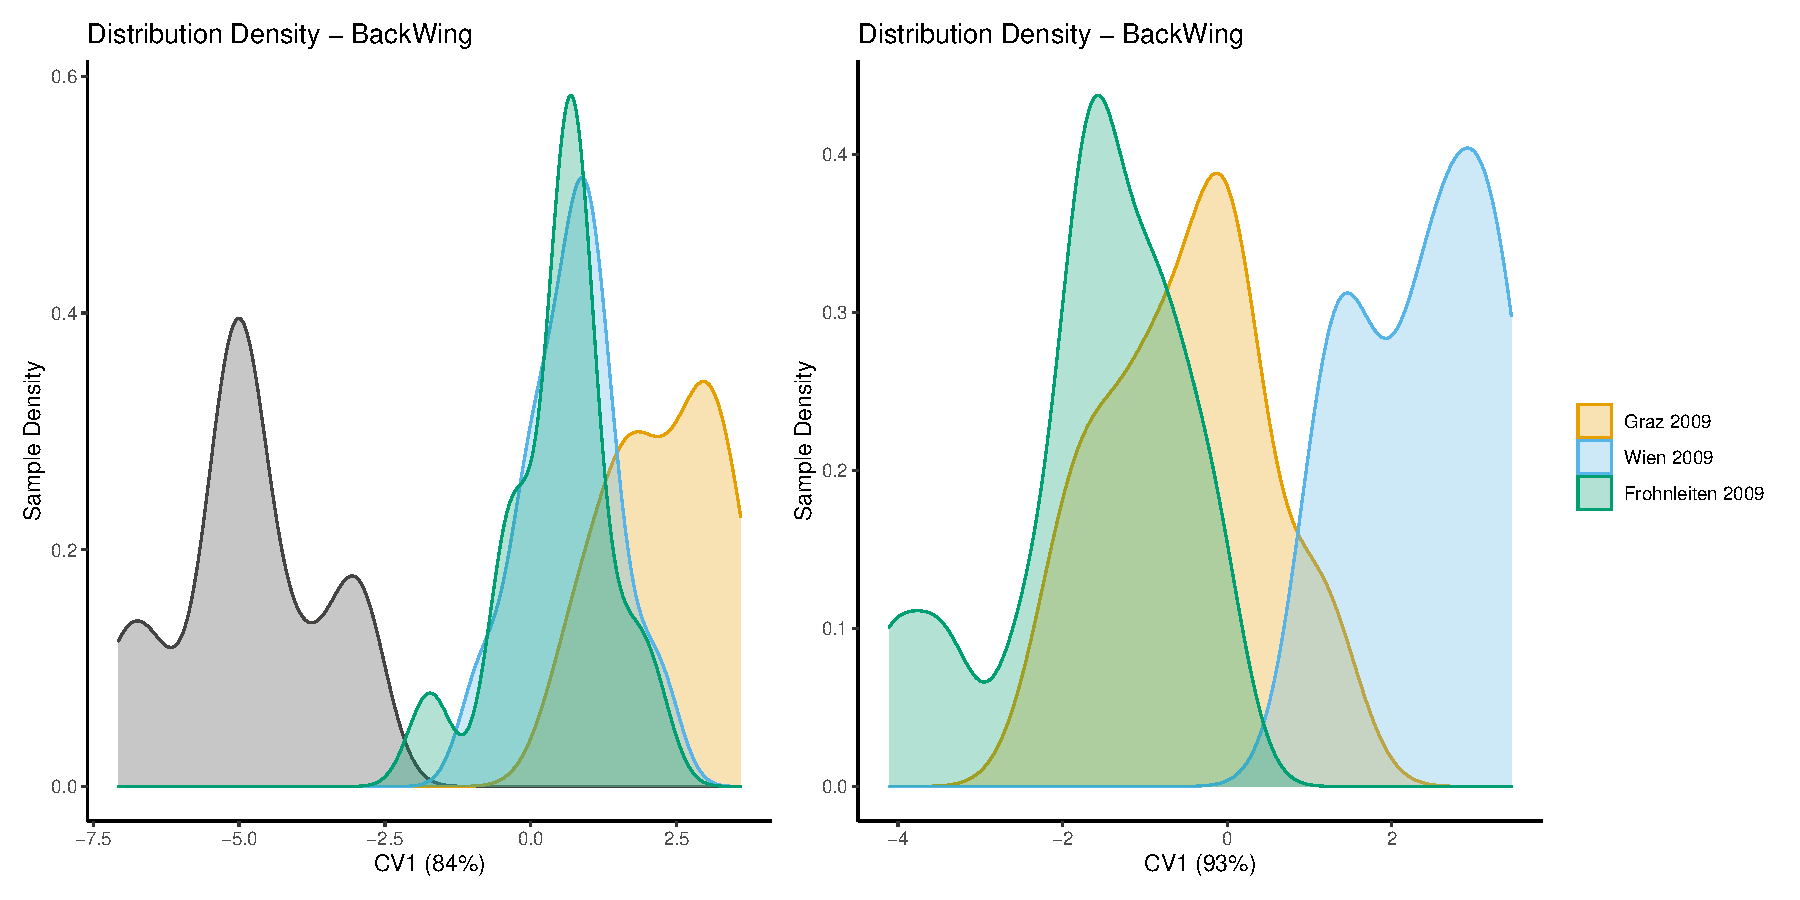
\includegraphics[width=0.8\linewidth,]{images/densPlot} 

}

\caption{Kernel density estimate of the samples for the first CVA dimension.}\label{fig:densCVA}
\end{figure}

With the CVA we can improve our differentiation of samples. Most of the between-sample variance is captured by the first dimension in both cases (fig.~\ref{fig:CVA}-\ref{fig:densCVA}). The accuracy of the CVA classification for the forewing 0.71 was better as for the backwing 0.6, see table \ref{tab:fwCVA} and \ref{tab:bwCVA}, but this may be biased because for the backwing the sample ``Graz 2011'' is missing.

\begin{table}

\caption{\label{tab:fwCVA}CVA leave-one-out cross-validation for the forewing, total accuracity 0.71.}
\centering
\begin{tabular}[t]{lrrrr}
\toprule
  & Graz 2011 & Graz 2009 & Wien 2009 & Frohnleiten 2009\\
\midrule
Graz 2011 & 9 & 0 & 1 & 0\\
Graz 2009 & 0 & 11 & 4 & 0\\
Wien 2009 & 0 & 1 & 8 & 3\\
Frohnleiten 2009 & 0 & 2 & 4 & 8\\
\bottomrule
\end{tabular}
\end{table}

\begin{table}

\caption{\label{tab:bwCVA}CVA leave-one-out cross-validation for the backwing, total accuracity 0.6.}
\centering
\begin{tabular}[t]{lrrr}
\toprule
  & Graz 2009 & Wien 2009 & Frohnleiten 2009\\
\midrule
Graz 2009 & 8 & 2 & 5\\
Wien 2009 & 2 & 10 & 0\\
Frohnleiten 2009 & 6 & 1 & 6\\
\bottomrule
\end{tabular}
\end{table}

\hypertarget{discussion}{%
\section{Discussion}\label{discussion}}

The centroid size (CS) is clearly different between our samples, see fig.~\ref{fig:csPlot}. The CS in winged insects could be seen as proxy for the actual body size, which was found in a study for damselflies (\protect\hyperlink{ref-outomuro2011}{Outomuro and Johansson 2011}). There are multiple reason why the absolute body size or the wing sizes may differ. One explanation could be genetics and as all worker bees in a colony are sisters the intra-sample variation is lower. Another explanation would be the size of the comb cells which is influenced by the cell size of the foundation made available by the beekeeper and also the age of combs, as for older combs the diameter of cells decreased, due to accumulated cocoons and fecal materials (\protect\hyperlink{ref-berry2001}{Berry and Delaplane 2001}). It could also indicate environment conditions as better nutrients availability probably results in more fed larvae or a visual precursor for underlying health conditions, as Varroosis can lead to deformation of abdomen or wings (\protect\hyperlink{ref-genersch2010}{Genersch et al. 2010}; \protect\hyperlink{ref-morawetz2019}{Morawetz et al. 2019}).

If we look at one well known traditional morphometrics measurement of the cubital index (CI) (\protect\hyperlink{ref-goetze1959}{Goetze 1959}), we can separate our sample into two groups, see fig.~\ref{fig:ciPlot}. With ``Graz 2011'' and ``Frohnleiten 2009'' having a higher CI on average and ``Graz 2009'' and ``Wien 2009'' a lower one All CI are in range for \emph{A. m. carnica}, based on \protect\hyperlink{ref-ruttner1988}{Ruttner} (\protect\hyperlink{ref-ruttner1988}{1988}). The traditional morphometrics includes normally more than one parameter, as in my example (\protect\hyperlink{ref-ruttner2000}{Ruttner, Pour Elmi, and Fuchs 2000}). A study on direct comparison between geometric morphometrics and traditional morphometrics showed only marginal better results for the geometric morphometrics approach (\protect\hyperlink{ref-tofilski2008}{Tofilski 2008}). Nowadays modern genetic methods have shown that traditional morphometrics alone is not always good enough to differentiate subspecies in honeybees (\protect\hyperlink{ref-groeneveld2020}{Groeneveld et al. 2020}).

In the principal component analysis (PCA) each point represent a unique shape of our specimen (shape space). The PCA does only differentiate the sample from ``Graz 2011,'' all other samples are more or less overlapping in the shown PCs for both fore- and backwing, see fig.~\ref{fig:fwPCA}-\ref{fig:bwPCA}. With the extrapolated TPS for the forewing, we see that most of the variance is explained by the height and top outline of the beewing. As the sample from ``Graz 2011'' seem to have a more round outline and a thinner shape compared to the other samples. The difference between the first and second PC is not as clear on the first glance as the overall theme is the same, with slimmer and wider shape, but there are few LM different, which does mean different wing vein lengths. Some sliding LM seem to also dominate the difference, the same can be said for the backwing. If the sliding LM differences represent a real shape difference or are only an artifact needs further investigation. Especially the backwing difference along the PC axes seems to be predominately defined by the sliding landmarks of the bee wing outline.

The classification with CVA (fig.~\ref{fig:CVA}), which maximizes the variance between sample means to the pooled variance within the samples, based on the first ten PC dimensions, for fore- and backwing respectively, did have an accuracy of prediction with leave-one-out cross-validation for the forewing of 71\% and for the backwing 60\%, see table \ref{tab:fwCVA}-\ref{tab:bwCVA}. The higher accuracy may not only due to better differentiation for the forewing per sé, with more LM and therefore more possibility of variation, but also due to the more different ``Graz 2011'' sample, which already did differentiate based on the first dimension in the PCA.

Even though, I cannot differentiate perfectly between given samples, I have to say that without background information on the collected specimens, it is hard to tell if I even should see a difference, they could also be strongly related colonies in terms of genetic or ecological conditions. It seems so far that geometric morphometrics was only used as tool for differentiation between subspecies or populations and no direct effect or cause of the beewing differences were discussed (\protect\hyperlink{ref-kandemir2009}{Kandemir et al. 2009}; \protect\hyperlink{ref-tofilski2008}{Tofilski 2008}; \protect\hyperlink{ref-francoy2006}{Francoy et al. 2006}). The missing discussion and visualization of shape is a great miss in my opinion, as it is one of the great benefits of geometric morphometrics (\protect\hyperlink{ref-mitteroecker2009}{Mitteroecker and Gunz 2009}). If the goal is only differentiation of populations based on ancestral history modern machine learning approaches on nucleotide polymorphisms seem to be very effective and highly efficient (\protect\hyperlink{ref-momeni2021}{Momeni et al. 2021}). Ofcourse here the advantage of geometric morphometrics would be the cheaper and more accessibility of the needed tools (\protect\hyperlink{ref-francoy2006}{Francoy et al. 2006}).

\hypertarget{references}{%
\section*{References}\label{references}}
\addcontentsline{toc}{section}{References}

\hypertarget{refs}{}
\begin{CSLReferences}{1}{0}
\leavevmode\hypertarget{ref-geomorph2021a}{}%
Adams, D. C., M. L. Collyer, A. Kaliontzopoulou, and E. Baken. 2021. {``Geomorph: Software for Geometric Morphometric Analyses. R Package Version 3.3.2.''} \url{https://cran.r-project.org/package=geomorph}.

\leavevmode\hypertarget{ref-berry2001}{}%
Berry, Jennifer A., and Keith S. Delaplane. 2001. {``Effects of Comb Age on Honey Bee Colony Growth and Brood Survivorship.''} \emph{Journal of Apicultural Research} 40 (1): 3--8. \url{https://doi.org/10.1080/00218839.2001.11101042}.

\leavevmode\hypertarget{ref-biesmeijer2006}{}%
Biesmeijer, J. C. 2006. {``Parallel Declines in Pollinators and Insect-Pollinated Plants in Britain and the Netherlands.''} \emph{Science} 313 (5785): 351--54. \url{https://doi.org/10.1126/science.1127863}.

\leavevmode\hypertarget{ref-francoy2006}{}%
Francoy, Tiago Maurício, Pedro Roberto Rodrigues Prado, Lionel Segui Gonçalves, Luciano da Fontoura Costa, and David De Jong. 2006. {``Morphometric Differences in a Single Wing Cell Can Discriminate {\emph{Apis Mellifera}} Racial Types.''} \emph{Apidologie} 37 (1): 91--97. \url{https://doi.org/10.1051/apido:2005062}.

\leavevmode\hypertarget{ref-gallai2009}{}%
Gallai, Nicola, Jean-Michel Salles, Josef Settele, and Bernard E. Vaissière. 2009. {``Economic Valuation of the Vulnerability of World Agriculture Confronted with Pollinator Decline.''} \emph{Ecological Economics} 68 (3): 810821. \url{https://doi.org/10.1016/J.ECOLECON.2008.06.014}.

\leavevmode\hypertarget{ref-genersch2010}{}%
Genersch, Elke, Werner von der Ohe, Hannes Kaatz, Annette Schroeder, Christoph Otten, Ralph Büchler, Stefan Berg, et al. 2010. {``The German Bee Monitoring Project: A Long Term Study to Understand Periodically High Winter Losses of Honey Bee Colonies.''} \emph{Apidologie} 41 (3): 332--52. \url{https://doi.org/10.1051/apido/2010014}.

\leavevmode\hypertarget{ref-goetze1959}{}%
Goetze, G. 1959. {``Die Bedeutung Des Flügelgeaders für züchterische Beuerteilung Der Honigbiene.''} \emph{Zeitschr. Bienenforsch.}, no. 4: 141--48.

\leavevmode\hypertarget{ref-goulson2013}{}%
Goulson, Dave. 2013. {``REVIEW: An Overview of the Environmental Risks Posed by Neonicotinoid Insecticides.''} Edited by David Kleijn. \emph{Journal of Applied Ecology} 50 (4): 977--87. \url{https://doi.org/10.1111/1365-2664.12111}.

\leavevmode\hypertarget{ref-grimaldi2005}{}%
Grimaldi, David, Michael S Engel, Michael S Engel, and Michael S Engel. 2005. \emph{Evolution of the Insects}. Cambridge University Press.

\leavevmode\hypertarget{ref-groeneveld2020}{}%
Groeneveld, L. F., L. A. Kirkerud, B. Dahle, M. Sunding, M. Flobakk, M. Kjos, D. Henriques, M. A. Pinto, and P. Berg. 2020. {``Conservation of the Dark Bee (Apis Mellifera Mellifera): Estimating C-Lineage Introgression in Nordic Breeding Stocks.''} \emph{Acta Agriculturae Scandinavica, Section A {{}} Animal Science} 69 (3): 157--68. \url{https://doi.org/10.1080/09064702.2020.1770327}.

\leavevmode\hypertarget{ref-hallmann2017}{}%
Hallmann, Caspar A., Martin Sorg, Eelke Jongejans, Henk Siepel, Nick Hofland, Heinz Schwan, Werner Stenmans, et al. 2017. {``More Than 75 Percent Decline over 27 Years in Total Flying Insect Biomass in Protected Areas.''} Edited by Eric Gordon Lamb. \emph{PLOS ONE} 12 (10): e0185809. \url{https://doi.org/10.1371/journal.pone.0185809}.

\leavevmode\hypertarget{ref-raster2020}{}%
Hijmans, Robert J. 2020. \emph{Raster: Geographic Data Analysis and Modeling}. \url{https://rspatial.org/raster}.

\leavevmode\hypertarget{ref-phylogen2020}{}%
Ilyasov, Rustem Abuzarovich, and Hyung Wook Kwon, eds. 2020. \emph{Phylogenetics of Bees}. Boca Raton, FL: CRC Press.

\leavevmode\hypertarget{ref-kandemir2009}{}%
Kandemir, İrfan, Mohammad G. Moradi, Berna Özden, and Ayça Özkan. 2009. {``Wing Geometry as a Tool for Studying the Population Structure of Dwarf Honey Bees (Apis Florea Fabricius 1876) in Iran.''} \emph{Journal of Apicultural Research} 48 (4): 238--46. \url{https://doi.org/10.3896/ibra.1.48.4.03}.

\leavevmode\hypertarget{ref-kearns1998}{}%
Kearns, Carol A., David W. Inouye, and Nickolas M. Waser. 1998. {``ENDANGERED MUTUALISMS: The Conservation of Plant-Pollinator Interactions.''} \emph{Annual Review of Ecology and Systematics} 29 (1): 83--112. \url{https://doi.org/10.1146/annurev.ecolsys.29.1.83}.

\leavevmode\hypertarget{ref-mitteroecker2009}{}%
Mitteroecker, Philipp, and Philipp Gunz. 2009. {``Advances in Geometric Morphometrics.''} \emph{Evolutionary Biology} 36 (2): 235--47. \url{https://doi.org/10.1007/s11692-009-9055-x}.

\leavevmode\hypertarget{ref-mitteroecker2013}{}%
Mitteroecker, Philipp, Philipp Gunz, Sonja Windhager, and Katrin Schaefer. 2013. {``A brief review of shape, form, and allometry in geometric morphometrics, with applications to human facial morphology.''} \emph{Hystrix, the Italian Journal of Mammalogy} 24 (1). \url{https://doi.org/10.4404/hystrix-24.1-6369}.

\leavevmode\hypertarget{ref-momeni2021}{}%
Momeni, Jamal, Melanie Parejo, Rasmus O. Nielsen, Jorge Langa, Iratxe Montes, Laetitia Papoutsis, Leila Farajzadeh, et al. 2021. {``Authoritative Subspecies Diagnosis Tool for European Honey Bees Based on Ancestry Informative SNPs.''} \emph{BMC Genomics} 22 (1). \url{https://doi.org/10.1186/s12864-021-07379-7}.

\leavevmode\hypertarget{ref-morawetz2019}{}%
Morawetz, Linde, Hemma Köglberger, Antonia Griesbacher, Irmgard Derakhshifar, Karl Crailsheim, Robert Brodschneider, and Rudolf Moosbeckhofer. 2019. {``Health Status of Honey Bee Colonies (Apis Mellifera) and Disease-Related Risk Factors for Colony Losses in Austria.''} \emph{Plos One} 14 (7): e0219293. \url{https://doi.org/10.1371/journal.pone.0219293}.

\leavevmode\hypertarget{ref-outomuro2011}{}%
Outomuro, Davi, and Frank Johansson. 2011. {``The Effects of Latitude, Body Size, and Sexual Selection on Wing Shape in a Damselfly.''} \emph{Biological Journal of the Linnean Society} 102 (2): 263--74. \url{https://doi.org/10.1111/j.1095-8312.2010.01591.x}.

\leavevmode\hypertarget{ref-potts2010}{}%
Potts, Simon G., Jacobus C. Biesmeijer, Claire Kremen, Peter Neumann, Oliver Schweiger, and William E. Kunin. 2010. {``Global Pollinator Declines: Trends, Impacts and Drivers.''} \emph{Trends in Ecology \& Evolution} 25 (6): 345--53. \url{https://doi.org/10.1016/j.tree.2010.01.007}.

\leavevmode\hypertarget{ref-r2020}{}%
R Core Team. 2020. \emph{R: A Language and Environment for Statistical Computing}. Vienna, Austria: R Foundation for Statistical Computing. \url{https://www.R-project.org/}.

\leavevmode\hypertarget{ref-rohlf2015}{}%
Rohlf, F. 2015. {``The tps series of software.''} \emph{Hystrix, the Italian Journal of Mammalogy} 26 (1). \url{https://doi.org/10.4404/hystrix-26.1-11264}.

\leavevmode\hypertarget{ref-RStudio2021}{}%
RStudio Team. 2021. \emph{RStudio: Integrated Development Environment for r}. Boston, MA: RStudio, PBC. \url{http://www.rstudio.com/}.

\leavevmode\hypertarget{ref-ruttner1988}{}%
Ruttner, Friedrich. 1988. \emph{Biogeography and Taxonomy of Honeybees}. Berlin, Heidelberg: Springer Berlin Heidelberg. \url{https://doi.org/10.1007/978-3-642-72649-1}.

\leavevmode\hypertarget{ref-ruttner2000}{}%
Ruttner, Friedrich, M. Pour Elmi, and Stefan Fuchs. 2000. {``Ecoclines in the Near East Along 36? N Latitude in Apis Mellifera l.''} \emph{Apidologie} 31 (2): 157--65. \url{https://doi.org/10.1051/apido:2000113}.

\leavevmode\hypertarget{ref-suxe1nchez-bayo2019}{}%
Sánchez-Bayo, Francisco, and Kris A.G. Wyckhuys. 2019. {``Worldwide Decline of the Entomofauna: A Review of Its Drivers.''} \emph{Biological Conservation} 232 (April): 8--27. \url{https://doi.org/10.1016/j.biocon.2019.01.020}.

\leavevmode\hypertarget{ref-tofilski2008}{}%
Tofilski, Adam. 2008. {``Using Geometric Morphometrics and Standard Morphometry to Discriminate Three Honeybee Subspecies.''} \emph{Apidologie} 39 (5): 558--63. \url{https://doi.org/10.1051/apido:2008037}.

\leavevmode\hypertarget{ref-MASS2002}{}%
Venables, W. N., and B. D. Ripley. 2002. \emph{Modern Applied Statistics with s}. Fourth. New York: Springer. \url{http://www.stats.ox.ac.uk/pub/MASS4/}.

\leavevmode\hypertarget{ref-tidyverse2019}{}%
Wickham, Hadley, Mara Averick, Jennifer Bryan, Winston Chang, Lucy D'Agostino McGowan, Romain François, Garrett Grolemund, et al. 2019. {``Welcome to the {tidyverse}.''} \emph{Journal of Open Source Software} 4 (43): 1686. \url{https://doi.org/10.21105/joss.01686}.

\leavevmode\hypertarget{ref-woodcock2017}{}%
Woodcock, B. A., J. M. Bullock, R. F. Shore, M. S. Heard, M. G. Pereira, J. Redhead, L. Ridding, et al. 2017. {``Country-Specific Effects of Neonicotinoid Pesticides on Honey Bees and Wild Bees.''} \emph{Science} 356 (6345): 1393--95. \url{https://doi.org/10.1126/science.aaa1190}.

\end{CSLReferences}

\end{document}
